\chapter{Introduction} \label{chap:intro}

%\version{v1.11.2015}

\section*{}
\section{Is computer science science?}
Is computer science, science? Yes, it is \cite{ICSS05}.

This is one of the most important chapters of the report. It should begin with a clear statement of what the project is about so that the nature and scope of the project can be understood by any reader. It should summarise everything you set out to achieve, provide a clear summary of the project's background, relevance and main contributions. The introduction should set the context for the project and should provide the reader with a summary of the key things to look out for in the remainder of the report. When detailing the contributions it is helpful to provide pointers to the section(s) of the report that provide the relevant technical details. The introduction itself should be largely non-technical. It is useful to state the main objectives of the project as part of the introduction. Should have the following headings:

\begin{itemize}
	\item Project Background/Overview
	\item Problem Description
	\item 	Project Objectives 
	\item Project Scope
\end{itemize}

\section{The Degree Project Report}
The project report is an extremely important aspect of the degree project. It should be properly structured and contain all the necessary and appropriate information regarding the project.
 
Project report has to be progressively developed as and when various stages of project are completed and last few weeks should be used to bring it together as a coherent document.

\textbf{A well structured and consistently formatted project report makes reading easier and is suggestive of a careful and professional attitude towards its preparation. }

Remember that quantity does not automatically guarantee quality. A 150 page report is not twice as good as a 75-page one, nor a 10,000 line implementation twice as good as a 5,000 line one. Conciseness, clarity and elegance are invaluable qualities in report writing, just as they are in programming, and will be rewarded appropriately. 

This document provides various guidelines for preparing a well structured project report.

\begin{figure}[t]
\centering
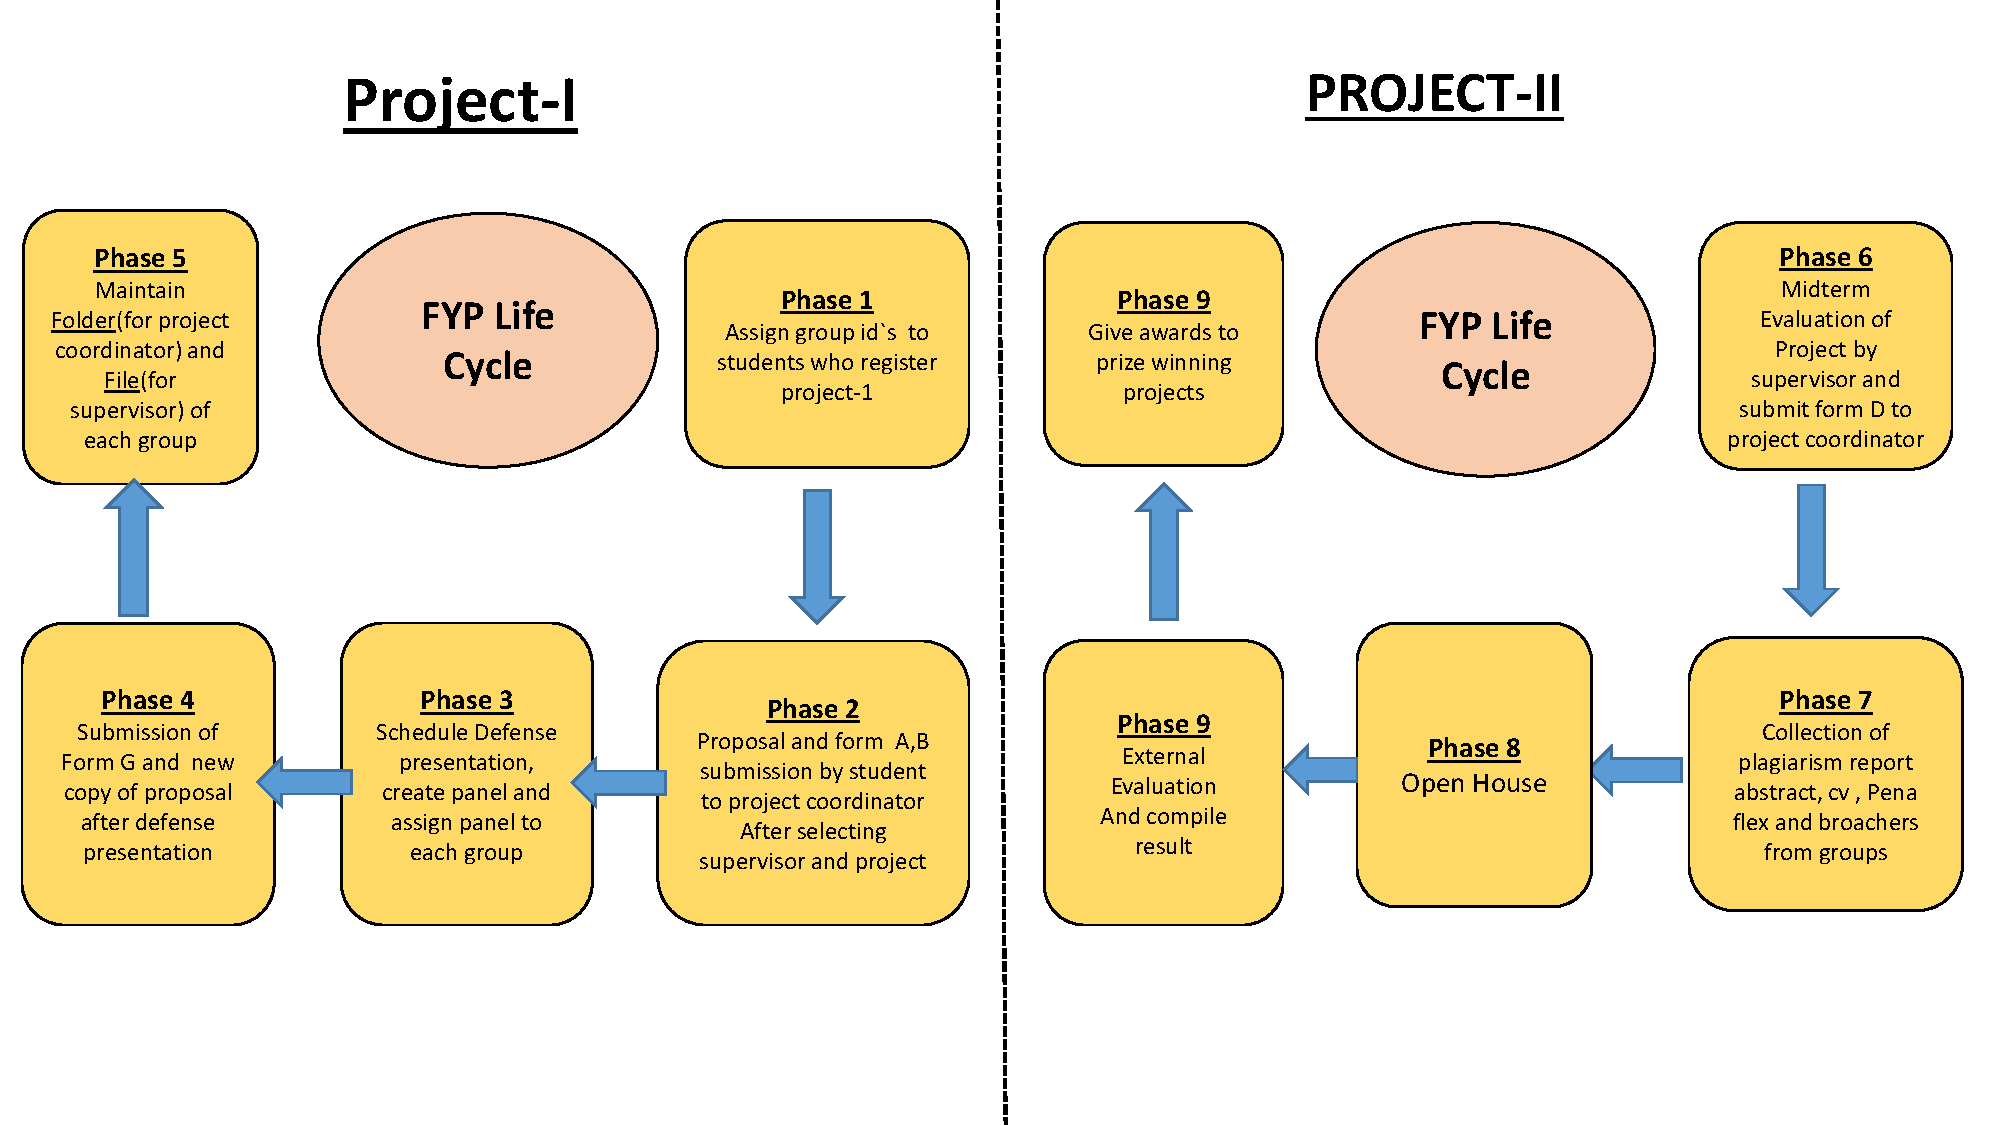
\includegraphics[scale=0.4]{fypLifeCycle}
\caption{Final Year Project Lifecycle}
\label{fig:fypLifeCycle}
\end{figure}

%%more details about figures can be found on https://en.wikibooks.org/wiki/LaTeX/Floats,_Figures_and_Captions
